\documentclass{sigchi}
%\documentclass[chi_draft]{sigchi}

% Use this section to set the ACM copyright statement (e.g. for
% preprints).  Consult the conference website for the camera-ready
% copyright statement.

% Copyright
%\CopyrightYear{2018} 
%\setcopyright{acmcopyright}
%\setcopyright{acmlicensed}
%\setcopyright{rightsretained}
%\setcopyright{usgov}
%\setcopyright{usgovmixed}
%\setcopyright{cagov}
%\setcopyright{cagovmixed}
% DOI
%\doi{http://dx.doi.org/10.475/123_4}
% ISBN
%\isbn{123-4567-24-567/08/06}
%Conference
%\conferenceinfo{IDC '18,}{June 19-23, 2018, Trondheim, Norway}
%Price
%\acmPrice{\$15.00}

\CopyrightYear{2018}
\setcopyright{acmlicensed}
\conferenceinfo{IDC '18,}{June 19--22, 2018, Trondheim, Norway}
\isbn{978-1-4503-5152-2/18/06}\acmPrice{\$15.00}
\doi{https://doi.org/10.1145/3202185.3202743}

% Use this command to override the default ACM copyright statement
% (e.g. for preprints).  Consult the conference website for the
% camera-ready copyright statement.

%% HOW TO OVERRIDE THE DEFAULT COPYRIGHT STRIP --
%% Please note you need to make sure the copy for your specific
%% license is used here!
 %\toappear{
 %Permission to make digital or hard copies of all or part of this work
 %for personal or classroom use is granted without fee provided that
 %copies are not made or distributed for profit or commercial advantage
 %and that copies bear this notice and the full citation on the first
 %page. Copyrights for components of this work owned by others than ACM
 %must be honored. Abstracting with credit is permitted. To copy
 %otherwise, or republish, to post on servers or to redistribute to
 %lists, requires prior specific permission and/or a fee. Request
 %permissions from \href{mailto:Permissions@acm.org}{Permissions@acm.org}. \\
 %IDC '18,  June 2018, Trondheim, Norway\\
 %ACM xxx-x-xxxx-xxxx-x/xx/xx\ldots \$15.00 \\
 %DOI: \url{http://dx.doi.org/xx.xxxx/xxxxxxx.xxxxxxx}
 %}

% Arabic page numbers for submission.  Remove this line to eliminate
% page numbers for the camera ready copy
% \pagenumbering{arabic}

% Load basic packages
\usepackage{balance}       % to better equalize the last page
\usepackage{graphics}      % for EPS, load graphicx instead 
\usepackage[T1]{fontenc}   % for umlauts and other diaeresis
\usepackage{txfonts}
\usepackage{mathptmx}
\usepackage[pdflang={en-US},pdftex]{hyperref}
\usepackage{color}
\usepackage{booktabs}
\usepackage{textcomp}
\usepackage{todonotes}
\usepackage{tipa}
\usepackage[french]{babel}
\usepackage{multirow}
\usepackage{amsmath}
\usepackage{calc}
\usepackage{graphicx}
\usepackage{subcaption}
\usepackage[none]{hyphenat}
\newcommand{\ts}{\textsuperscript}
\usepackage[utf8]{inputenc}

%\usepackage[utf8x]{inputenc}

% Some optional stuff you might like/need.
\usepackage{microtype}        % Improved Tracking and Kerning
% \usepackage[all]{hypcap}    % Fixes bug in hyperref caption linking
\usepackage{ccicons}          % Cite your images correctly!
% \usepackage[utf8]{inputenc} % for a UTF8 editor only

% If you want to use todo notes, marginpars etc. during creation of
% your draft document, you have to enable the "chi_draft" option for
% the document class. To do this, change the very first line to:
% "\documentclass[chi_draft]{sigchi}". You can then place todo notes
% by using the "\todo{...}"  command. Make sure to disable the draft
% option again before submitting your final document.
%\usepackage{todonotes}

% Paper metadata (use plain text, for PDF inclusion and later
% re-using, if desired).  Use \emtpyauthor when submitting for review
% so you remain anonymous.
\def\plaintitle{When Deictic Gestures in a Robot Can Harm \\Child-Robot Collaboration}



\def\plainauthor{First Author, Second Author, Third Author,
  Fourth Author}
\def\emptyauthor{}
\def\plainkeywords{Child robot interaction; education; reading; learning by teaching; protégé effect; deictic gestures; pointing.}
\def\plaingeneralterms{Documentation, Standardization}

% llt: Define a global style for URLs, rather that the default one
\makeatletter
\def\url@leostyle{%
  \@ifundefined{selectfont}{
    \def\UrlFont{\sf}
  }{
    \def\UrlFont{\small\bf\ttfamily}
  }}
\makeatother
\urlstyle{leo}

% To make various LaTeX processors do the right thing with page size.
\def\pprw{8.5in}
\def\pprh{11in}
\special{papersize=\pprw,\pprh}
\setlength{\paperwidth}{\pprw}
\setlength{\paperheight}{\pprh}
\setlength{\pdfpagewidth}{\pprw}
\setlength{\pdfpageheight}{\pprh}

% Make sure hyperref comes last of your loaded packages, to give it a
% fighting chance of not being over-written, since its job is to
% redefine many LaTeX commands.
\definecolor{linkColor}{RGB}{6,125,233}
\hypersetup{%
  pdftitle={\plaintitle},
% Use \plainauthor for final version.
%  pdfauthor={\plainauthor},
  pdfauthor={\emptyauthor},
  pdfkeywords={\plainkeywords},
  pdfdisplaydoctitle=true, % For Accessibility
  bookmarksnumbered,
  pdfstartview={FitH},
  colorlinks,
  citecolor=black,
  filecolor=black,
  linkcolor=black,
  urlcolor=linkColor,
  breaklinks=true,
  hypertexnames=false
}
%
\def\sharedaffiliation{%
\end{tabular}
\begin{tabular}{c}}
%
% create a shortcut to typeset table headings
% \newcommand\tabhead[1]{\small\textbf{#1}}

% End of preamble. Here it comes the document.
\begin{document}

\title{\plaintitle}

\numberofauthors{4}
    \author{ Elmira Yadollahi $^{\star\dagger}$, Wafa Johal$^{\star}$, Ana Paiva$^{\dagger}$, Pierre Dillenbourg$^{\star}$\\      
%      
      \sharedaffiliation
      \affaddr{$^{\star}$École Polytechnique Fédérale de Lausanne, Switzerland}  \\
      \affaddr{$^{\dagger}$Instituto Superior Técnico, University of Lisbon, Portugal}   \\
      \email{elmira.yadollahi@epfl.ch,}     
      \email{wafa.johal@epfl.ch,}  
      \email{ana.paiva@inesc-id.pt,} 
      \email{pierre.dillenbourg@epfl.ch}
          }
%
\maketitle


\begin{abstract}
%Reading is considered a fundamental and crucial aspect of learning, leading to the acquisition of language, social, and critical thinking skills.
%While the school systems are designed to provide the fundamentals of reading and related training, repeated practices in school and at home are essential to master this skill, especially for children with reading difficulties. 
This paper describes research aimed at supporting children's reading practices using a robot designed to interact with children as their reading companion.
We use a learning by teaching scenario in which the robot has a similar or lower reading level compared to children, and needs help and extra practice to develop its reading skills. 
The interaction is structured with robot reading to the child and sometimes making mistakes as the robot is considered to be in the learning phase. 
Child corrects the robot by giving it instant feedbacks. 
To understand what kind of behavior can be more constructive to the interaction especially in helping the child, we evaluated the effect of a deictic gesture, namely pointing on the child's ability to find reading mistakes made by the robot. 
We designed three types of mistakes corresponding to different levels of reading mastery.
We tested our system in a within-subject experiment with 16 children.
We split children into a high and low reading proficiency even-though they were all beginners.
For the high reading proficiency group, we observed that pointing gestures were beneficial for recognizing some types of mistakes that the robot made.
For the earlier stage group of readers pointing were helping to find mistakes that were raised upon a mismatch between text and illustrations. 
However, surprisingly, for this same group of children, the deictic gestures were disturbing in recognizing mismatches between text and meaning.



\end{abstract}


\begin{CCSXML}
<ccs2012>
<concept>
<concept_id>10010405.10010489.10010492</concept_id>
<concept_desc>Applied computing~Collaborative learning</concept_desc>
<concept_significance>500</concept_significance>
</concept>
<concept>
<concept_id>10003120.10003121.10011748</concept_id>
<concept_desc>Human-centered computing~Empirical studies in HCI</concept_desc>
<concept_significance>300</concept_significance>
</concept>
<concept>
<concept_id>10003120.10003123.10011759</concept_id>
<concept_desc>Human-centered computing~Empirical studies in interaction design</concept_desc>
<concept_significance>300</concept_significance>
</concept>
</ccs2012>
\end{CCSXML}

\ccsdesc[500]{Applied computing~Collaborative learning}
\ccsdesc[300]{Human-centered computing~Empirical studies in HCI}
\ccsdesc[300]{Human-centered computing~Empirical studies in interaction design}

\printccsdesc

%\category{H.5.m.}{Information Interfaces and Presentation
%  (e.g. HCI)}{Miscellaneous} \category{See
%  \url{http://acm.org/about/class/1998/} for the full list of ACM
%  classifiers. This section is required.}{}{}

\keywords{\plainkeywords}


\begin{figure}[t]
  \centering
  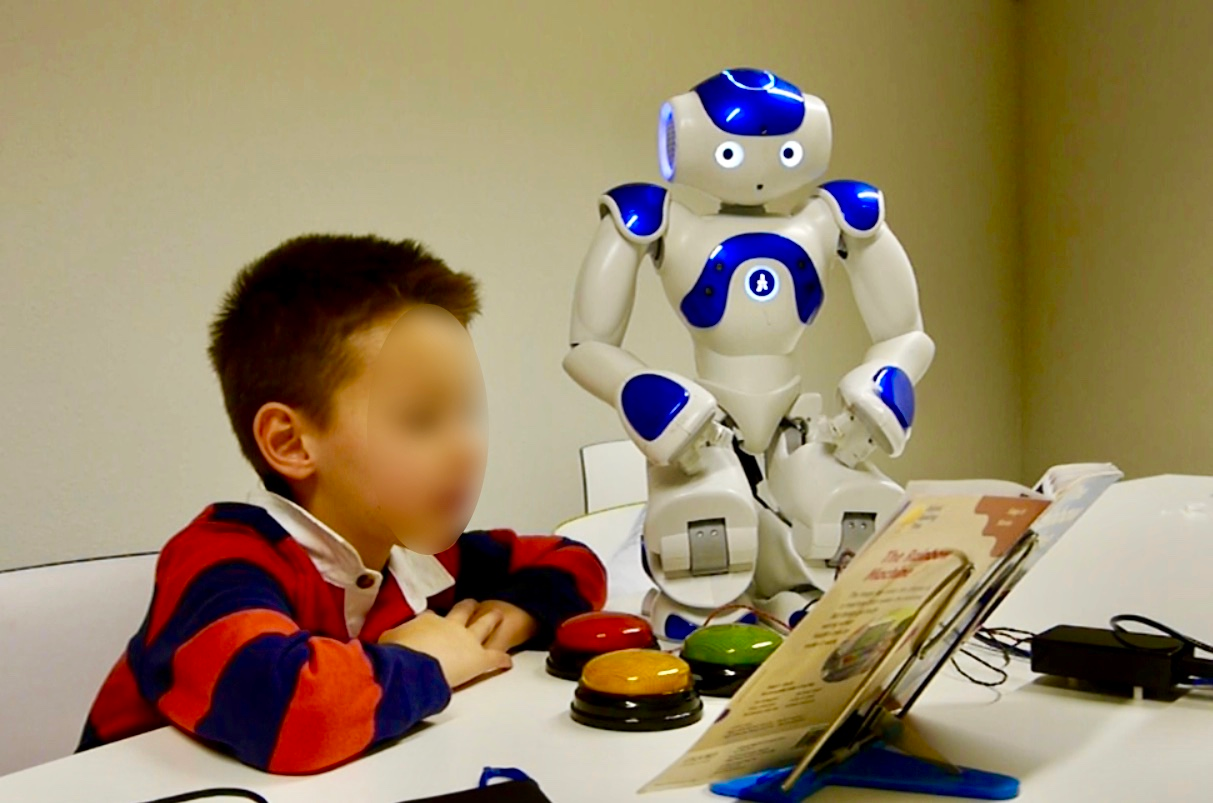
\includegraphics[width=1\linewidth]{figures/Expsetup2.png}
  \caption{CoReader Activity Platform}
  \label{fig:readingExp}
\end{figure}

\section{Introduction}
Reading is considered a fundamental and crucial aspect of learning, leading to the acquisition of language, social, and critical thinking skills.
While the school systems are designed to provide the fundamentals of reading and related training, repeated practices in school and at home are essential to master this skill, especially for children with reading difficulties. 
Previous studies suggest that the experience acquired by children in early stages of life has a long-lasting impact on their development \cite{feldman2008early}. 
Failing or encountering difficulties in learning literacy can affect the child emotionally. 
This issue can be addressed or prevented, and some of the ways for boosting children's self-esteem is to make sure they receive genuine praise based on their success \cite{valiente2012linking}.
It is evident that in each class, children learn at different paces and they usually show different levels of progress. 
Managing children with heterogeneous levels requires either adjusting the material to the child's level (also called differentiation \cite{van1996isomorphism}) or keeping the higher level children within the class average and pushing the lower level ones to catch up \cite{schmeck2013learning}.
Either method has its own advantages and disadvantages and can create frustration in children who are behind their peers. 
Children with reading difficulties require more practice and exposure to reading materials \cite{reid2016dyslexia}. 
These extra practices should be constructive in both technical and emotional aspects. 

One type of additional practices provided for children with difficulties in reading is individual or small group tutoring. 
Currently, the majority of tutoring is delivered by teachers or skilled peer tutors \cite{wood1976role,goodlad1989peer,wenger2014artificial}. 
Concurrently, there are some emerging new studies providing individual and adaptive tutoring to children using social robots \cite{belpaeme2015l2tor,leyzberg2014personalizing,brown2013engaging}.
%
In this context, robots have been used as a teacher/tutor, learning companion, and learner in different educational scenarios and with varying learning goals.
Presently, there are numerous works dedicated to studying the effects of robot tutors in social robotics \cite{kanda2004interactive, castellano2009detecting,ribeiro2014m,kennedy2015robot}.
On the other hand, little work has been done to study the effect of learning by teaching paradigm in development of reading proficiency. 
However, the use of learning by teaching paradigm has been explored and studied in different fields such as writing and biology \cite{hood2015children,chase2009teachable}.

It is known that designing learning activities with robots requires a precise understanding of the robot's role and its implications for learning, in our case reading.
Nevertheless, it is important to precisely define the role of the robot and its effect on reading, which requires a proper discernment of the reading skill. 
Reading is a composition of a variety of complex cognitive performances with discrete yet interdependent mental processes \cite{kirby1988style}.  
According to Kirby \cite{kirby1988style} reading in any instance is a function of task difficulty, reader's skills, and reader's purpose. 
Hence,  our interaction design should take into account all of these factors.  


% CONTRIBUTION SECTION
This paper presents the design of a platform to engage children in a reading while listening (RWL) activity, with the robot reading the text and the child helping the robot in case of making mistakes.
The idea is to use learning by teaching paradigm to keep the child motivated and interested in the interaction.
However, in our proposed user study, we intend to explore the effect of robot's deictic gestures during reading on the child. 
The interaction is designed in a way that the robot makes mistakes and the child corrects them.
We want to see how much a deictic gesture such a pointing to text can help the child's reading while listening (RWL) proficiency. 
The effect of pointing on the child's reading, especially on children with reading difficulties and poor readers can provide valuable information in designing reading companions for children. 
We believe understating this effect can be a building block of designing our reading platform, and informative as to know when and how the robot should use deictic gestures during reading. 


In the following sections, first, we present the previous works in human-robot interaction and education alongside the studies that have inspired the hypotheses of our work. 
Then, we describe the design of our reading platform explaining how the robot and interaction are implemented. 
After that, we demonstrate the design of our experiment with details about participants, selection of reading materials, design of mistakes, robot's behaviors and our research hypotheses. 
Then we present the evaluation of our results for each hypothesis. 
In the final sections, we discuss the results, reflect on the teacher's and children's input, explain the limitations of our work, provide the future developments of our platform, and describe our contributions.




\section{Related Works}


Our study describes the development of a reading activity within a child-robot interaction scenario while it incorporates learning by teaching paradigm.
Aligned with developing the robots cognitive abilities, we designed a user study to evaluate the effect of robot's deictic gestures such as pointing to text on the child's reading. 
As a result, we present a review of relevant works done in the field of robots in education and implementations of learning by teaching paradigm in human-robot interaction. 
Moreover, we look at recent studies on reading and storytelling with a robot.
Meanwhile, we also discuss studies on reading detailing methods to evaluate and help children with difficulties.
Finally, we give a quick review of the studies evaluating the effect of pointing gestures on learning and performance.

\subsection{Robots in Education}
In the conjunction of human-robot interaction and education, the role of the robots can vary from being a tool for learning certain subjects to agents that accompany the learner in learning environments. 
Looking closely, it is evident that robot can take on different roles to teach, assist, inspire and motivate the learner. 
Therefore, a robot can take on the role of a teacher or tutor, a learning companion, or a learner \cite{mubin2013review,leite2013social,hood2015children}. 
A study by Kanda et al. \cite{kanda2004interactive} using robots as peer English tutors shows different ways children interact with robots and can benefit from them. 
Long-term interaction studies by Tanaka et al. using QRIO \cite{tanaka2007socialization} and Hyun et al. using iRobiQ \cite{hyun2010relationships}, show the level of social interactions between the robot and children. 
Through these experiments, they provide guidelines for using robots as tutors in the classrooms.
On another study by Leyzberg et al. \cite{leyzberg2014personalizing} the effect of personalization of a tutor robot on the students' performance was evaluated. 
L2TOR by Belpaeme et al. \cite{belpaeme2015l2tor} is a recent project focusing on evaluating social robots for tutoring second language to children in early childhood .
L2TOR project tries to address current demands and define the pedagogy of a robot-assisted tutoring. 
Learning a certain subject during the interaction with robots has also been studied \cite{brown2013engaging,hood2015children}. 
In Brown's study \cite{brown2013engaging} they used a robot; Darwin, to assist children in solving math questions.
In the other hand, hood's study \cite{hood2015children, lemaignan2016learning} introduced the CoWriter project focusing on writing activities using the robot Nao.
CoWriter is a project that motivates children to help a robot with bad handwriting, and in the process, it engages children into practicing their own handwriting in a more subtle yet productive way as they feel responsible to help the robot. 
This phenomenon is called protégé effect which emerges through learning by teaching paradigm.  

\subsection{Learning by Teaching}

Previous research in education and cognitive sciences suggests that one of the powerful methods of learning is teaching others \cite{bargh1980cognitive}.
The potential of learning by teaching can also be deduced from methods such as peer-assisted tutoring, reciprocal teaching, small group interaction, and self-explanation each of which possesses a certain degree of teaching to others. 
There is also research demonstrating the positive effect of learning by teaching in computer-assisted learning environments \cite{biswas2005learning,chase2009teachable}. 
The effect of using teachable agents during learning activities, on motivation and learning gain of the students have been studied by Chase et al. \cite{chase2009teachable}. 
They observed students who taught to the teachable agents spent more time on learning behaviors and learned more than students who learned by themselves.
Besides, they observed that protégé effect was particularly more helpful to low-achieving students. 
As a result, an adoption of protégé effect in learning can bring an intrinsic level of motivation combined with a sense of responsibility for the robot, which can change the experience of learning. 

\subsection{Reading and Storytelling}
Concerning reading activities, there have been multiple studies focusing on reading or storytelling activities with children aiming to make it more engaging \cite{rubegni2016evaluating}. 
Storytelling activities consist of telling a story by focusing on education or entertainment or creating a story based on available or given elements.
These studies can be divided into three categories: 1) when the robot is reading or telling a story, 2) when the child is reading or telling the story, or 3) when someone else is reading to both of them. 

One method suggested to help children with reading difficulties is \textit{Reading While Listening} (RWL). 
The effect of RWL is shown to be promising for poor readers in improving comprehension, word recognition, reading fluency, acquisition of word meaning, and learning to read \cite{carbo1978teaching,chomsky1976after}. 
One of the latest studies devising synchronized RWL is by Gerbier et al. \cite{gerbier2018audio}. 
They evaluate the effect of visually highlighting the text as it is being read compared to simple text condition.
Their study shows that poor readers tend to benefit more from these visual cues.
Another recent example of technology used to assist readers is PhonoBlocks, a Tangible User Interface (TUI) for children with dyslexia \cite{fan2016design}.
In studies using robots, the work by Michaelis and Mutlu \cite{michaelis2017someone} proposes an in-home learning companion, in which the child is reading to a robot. 
They focus on how such companion can help children to expand their reading interests and abilities. 
\textit{Family Story Play} is another reading platform that uses a digital companion for long-distance reading interaction between children and grandparents \cite{raffle2010family}.  
To facilitate the interaction, the platform uses a digital social agent in the form of Elmo to help enriching the interaction between the child and grandparents and strengthening dialogic reading. 
Storytelling delves into another aspect of interaction with a robot. 
For a robot to be a good storyteller being aware of its audience is critical.
The study by Mutlu et al. \cite{mutlu2006storytelling} shows how the robot's gaze behavior during storytelling affects the audience's perception of the robot.
Another system providing interactive storytelling is \textit{AIBOStory} which aims to enrich remote communication experiences on the Internet using AIBO robots \cite{papadopoulos2013aibostory}.
In the study by Kory and Breazeal \cite{kory2014storytelling}, a social robot interacts with children as a peer and plays a storytelling game with them.
The interaction is designed to introduce children to new vocabularies in the context of storytelling games. 
It evaluates the effect of adapting robot's language level to the child's learning, complexities of the stories, and similarities to the robot's stories.

%new part
Studies by Pellegrini and Brody \cite{pellegrini1985parents} and Bus et al. \cite{bus1995joint} show that parent-child shared book reading can be beneficial for the children's emergent literacy.
However, there are various factors that affect the interaction and its quality, such as the child's level of competence or parent's level of adjustment to the child's needs and problems.
These factors makes it hard to distinguish between the effect of parent's behavior on the child or child's behavior on the parent \cite{pellegrini1985parents}.  
MacNeil \cite{mcneill1992hand} and de Ruiter \cite{de200014} have a typology distinguishing different types of gestures used during speech or interaction. 
Among the different gestures that accompanies human speech, we are interested in deictic gestures that translates to pointing gestures during book reading.
Looking at the study by Justice et al. \cite{justice2008influence}, they examine the effect of verbal and nonverbal references by adult during storybook reading on children's visual attention to the print. 
The nonverbal references in their case translate to pointing to the print by tracking the text while reading.
Their study was conducted with preschool children, concluding that explicit referencing such as pointing increases the children's visual attention to the print. 

\setlength{\parskip}{2em}

While the majority of previous works consider the robot as a learning companion, Kory \cite{kory2014storytelling} found that the robot with lesser ability can trigger teaching and mentoring behaviors from children.
This behavior is aligned with the studies of the CoWriter project and the teachable agents by Chase et al. \cite{hood2015children,chase2009teachable}.
Our project's aims to motivate and inspire children to practice more, to challenge them, and to improve their self-confidence especially for children with reading difficulties. 
Our robot plays the role of a learning companion, which encompasses the learning by teaching paradigm within its premises.  
When the robot is reading to children, the idea of correcting the robot pushes children to read alongside it, which creates a Reading While Listening (RWL) experience.
While none of the previous works concerning reading and storytelling in robotics studied the effect of pointing with a robot, a study by Sharma et al. \cite{sharma2016visual} analyzed the effect of deictic gestures on video lectures from MOOC . 
In their study, they investigate if augmenting a video with deictic gestures or with the teacher's gaze could increase the students' learning gain. They obtained significant results for the gaze cues only but the deictic modality also showed higher student performances.
In this study, we use this learning by teaching setting to explore specifically the effect of robot's deictic gestures on the child's concentration of the reading task. 
To evaluate it, we use the proportion of correctly identified robot's mistakes as a measure of child performance.






\section{Design of the CoReader Platform}

The CoReader platform, shown in Figure \ref{fig:readingPlatform} supports the collaborative reading of stories between a child and a robot. 
The platform consists of a Nao robot, a paper book, and three tangible feedback buttons.
During the interaction, child and robot are sitting beside each other facing a book at an angle between 30 to 50 degrees, which is considered to be a side-by-side F-formation \cite{kendon1990conducting}.
The interaction is designed to be simple and understandable for children. 
The robot interacts with the child and reads the chosen book, sometimes with mistakes. To correct the mistakes of the robot the child can use the buttons. 
At some point the child can also read the book.

The whole system is implemented using the Robotic Operating System (ROS) and is totally autonomous.
The use of \textit{Augmented Reality Tags} ARTags package \footnote{\href{http://wiki.ros.org/ar_track_alvar}{AR Track Alvar from ROS}} allows a flexible selection of books, as really few and simple modifications are required for each book (sticking the visual tags), beside associating the book text to the corresponding visual tag. 
It also implies low costs as neither complicated programming nor costly modification of the books is required.
\begin{figure}[t]
  \centering
  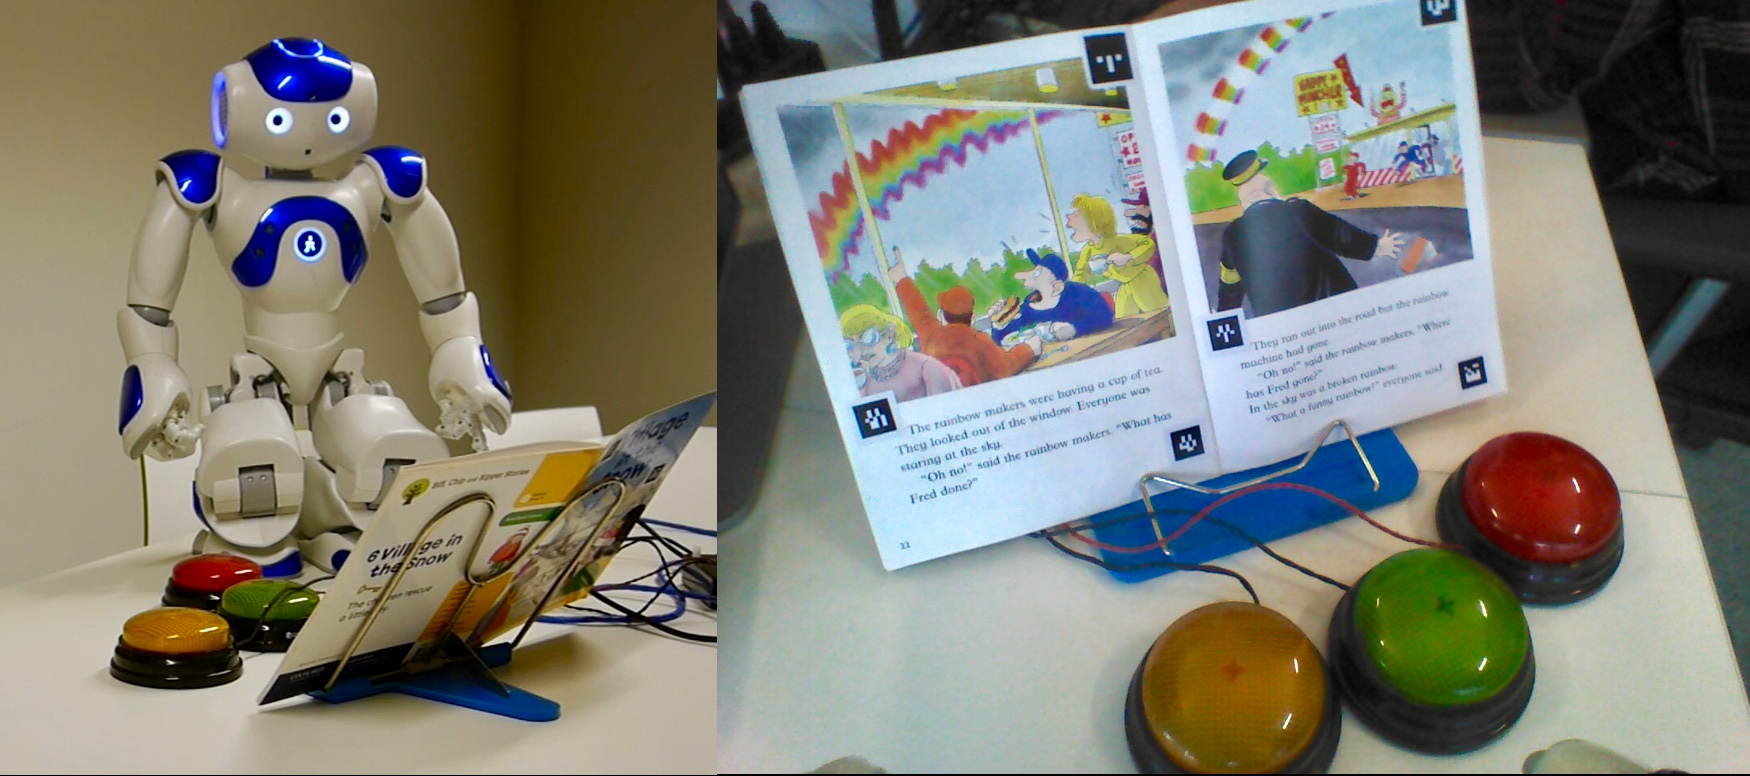
\includegraphics[width=1\linewidth]{figures/booknrobot2.png}
  \caption{CoReader platform; Left image shows the robot with the book and buttons; Right image shows the view from the robot's bottom camera looking at the book accompanied with ARTags}
  \label{fig:readingPlatform}
\end{figure}

The feedback buttons are placed in front of the child to facilitate his/her interaction with the robot as shown in figure \ref{fig:readingExp}. 
It provides actions such as informing the robot of its mistakes (red button), asking the robot to repeat a page (yellow button) and giving positive feedback to the robot (green button). 
Red button can be pressed at any moment when the robot is reading to inform about mistakes. 
Right after receiving a signal from the red button, robot reacts to its mistake by verbal, physical, and emotional gestures (through changing eye color). 
The child informs the robot of the correct word and then the robot repeats reading the page, this time correcting its mistake. 
The yellow button, for repeating, can also be pressed at any time. 
After receiving a \emph{repeat} signal, the robot stops reading in case it was in the middle of the text and repeats from the start of the page. 
The green button can be used at the end of each page to inform and praise the robot of its success when it doesn't make any mistake. 
Pressing this button is followed by robot's reaction with happy verbal, physical, emotional gestures.


The robot can express itself through a mixture of verbal and expressive actions which are a combination of the robot's movement and dialogues acts. These allow for the robot to express its understanding of making a mistake and its happiness of being correct after being praised.
To convey an emotional response of each reaction, we use the robot's eyes to imitate human emotions, considering that the Nao robot cannot render facial expressions. 
For this purpose, we apply the LED patterns created and evaluated by Johnson et al. \cite{johnson2013imitating} allowing to express six basic emotions. In our study we only use \emph{surprise} and \emph{sadness} for reactions after making a mistake and \emph{happiness} for reactions after being praised.

The interaction as a whole was designed to be simple and understandable for children. 
In the beginning of each session, the robot introduces itself, expresses its desire to read the book, but it also explains that sometimes it needs help when it makes mistakes. 
Before the start of the interaction, each child is informed of how the interaction flows, how to use the buttons, and his/her role in helping and correcting the robot in case of making mistakes.
If the robot makes a mistake and the child doesn't recognize it, the robot keeps that state in memory and makes that mistake again if it is asked to repeat the page afterwards.
For assessment purposes, the child is not informed about the mistakes that he/she didn't recognize, and the interaction will be carried out regardless of recognition of mistakes.


\section{Experiment Design}
\subsection{Participants}
The study involved 22 typically developing children between the age of 6 and 7 (11F, 11M) selected from second grade in an international school in Switzerland, participated in a within-subject experiment. Each child interacted with the robot during two sessions of around 30 minutes in two different days. 
The children were divided into two groups according to their reading level by their teacher. We refer to these two groups as \textit{Low} and \textit{High} level. 
We used the Oxford Reading Tree series to assign an appropriate book to each group based on their reading level (\textit{Low}: stage 4 of Oxford Reading Tree and \textit{High}: stage 7 of Oxford reading tree). 
According to the teacher, as soon as children in the Low level are proficient in their level they are promoted to the higher levels.
The \textit{Low} group consists of 9 children (5F, 4M) and \textit{High} level of 13 children (5F, 8M).

%new section
Regarding the children's profile participating in this experiment, all of them were selected from the same class, working with the same teacher. 
This is important in a sense that they were exposed to the same learning methods.
The separation of the children into two groups were based on the teachers assessment of their reading skills. 
However, such separation only exists in the class during reading sessions to adjust the level of the book to the child.
According to the teacher, ``pointing gestures were instinctively used to direct the children’s attention as they decode words and then sentences''.
``At the beginning it is very important to guide the children through the reading process.''
Most children drop the pointing technique as they become more confident readers. 
Although, children with attention problem would still benefit from this technique. 
And while all children are used to the pointing technique, some need the teacher to use pointing, some use their own fingers to point as they decode, and some don't seem to need it at all.


\subsection{Reading Material}
The books were selected after discussion with the primary school teacher and based on the children's reading levels and potentials.
Considering the design of the experiment, we selected a book one stage higher than the current level of the children for three reasons.
Firstly, to make the book challenging for the children; 
secondly, to keep children more interested in the activity, considering that it is easier to follow text when someone else is reading it for you; and finally
to make sure that the child had not read the book before. 

For the \textit{Low~level} group, a book from stage 5 of the Oxford Reading Tree with 24 illustrated pages was selected \footnote{Oxford Reading Tree Stage 5: \textit{Village in the Snow}; created by Roderick Hunt and Alex Brychta}.
It was divided into two equal parts, one was read on the first day of the experiment and the other on the second day. 
On Day 1,  the robot was reading 9 pages of the book and upon reaching the 10\ts{th} page, it announced to be tired and asked the child to continue reading until page 12\ts{th}. 
In the second day of the experiment, the robot welcomed back the child and showed its excitement to know the end of the story. 
In the same manner, robot read 9 pages and the child finished to read the 3 remaining pages of the book. 
The same procedure was carried out for the \textit{High-level group}, except that they read a stage 8\ts{th} book, with 32 pages \footnote{Oxford Reading Tree Stage 8: \textit{The Rainbow Machine}; created by Roderick Hunt and Alex Brychta}. 
With the same principle, robot reads 10 pages of the book and the child read the rest of the book until page 16 on the first day (and the same number on the second day until the end of the book).


\subsection{Mistakes Design}

The goal of the scenario is to engage children in reading with the robot while challenging them to read the text alongside and at the same time correct it. To achieve this, the robot should make mistakes while reading, to give the opportunity for the child to correct it. As such, the design of the mistakes made by the robot was an important part of our work. 
We considered that the robot should exhibit  similar mistakes as a child with reading difficulties. As such, we relied on to the body of work on \emph{Miscue Analyses} by Kenneth Goodman \cite{goodman1969analysis,goodman1973miscue} where  a taxonomy to analyze the readers' deviations from the text (called miscues) was proposed.
%The deviation from the text is labeled as \textit{miscue} and it is analyzed using 28 linguistic questions that investigate its compatibility with the text.
%The taxonomy was transformed into a diagnostic kit named \textit{Reading Miscue Inventory} (RMI) by Yetta Goodman and Burke \cite{goodman1972reading}.
%This inventory includes the guide to mark, select and code the miscues for further analyses.
%While RMI provides a diagnostic tool for reading clinicians or special reading teachers, it also has several disadvantages regarding the time needed for administration, scoring and interpreting the result. 

According to the \textit{Simplified Miscue Analysis} (SMA) by Cunningham \cite{cunningham1984simplified} %consists of steps to collect and code the 
miscues made by a reader can be analyzed through 4 questions. We used the first 3 questions from SMA to design our robot's mistakes. 

The questions from SMA examine the miscues based on similarity to the original wording, change in syntax, and change in meaning. 
These questions led us to define a property called the level of mismatch in designing the robot's mistake.
Furthermore, since we are working on books with images, we are also interested in adding a type of mistakes defined as a mismatch with illustrations. 
This type of mistake was added to check the children's attention to the illustrations and the reading, and they are easier to recognize. 
As a result we designed 3 types of mistakes based on the different types of mismatch.

\textbf{Type-1} mistakes are defined as any mismatch between the wording and the book's illustrations.
An example of this type is when the robot reads \textit{elephant} instead of \textit{penguin} while there is an image of a penguin in the book. 

\textbf{Type-2} mistakes (question 3 from SMA) are contextual mistakes and correspond to a change in the meaning of the sentence after being replaced with another word.
One example is saying  \textit{start} instead of \textit{stop} in the text. 
Mistakes of Type-1 can also change the context at times, but since they are recognizable through images, the priority is to categorize them as Type-1.

\begin{table}[t]
  \centering
  \footnotesize
  \renewcommand{\arraystretch}{1.8}
  \begin{tabular}{ |p{1.1cm} | p{2.1cm} | p{2.6cm}| p{1.1cm} | }
          \hline
          
          \textbf{Mistake Type} & \textbf{Description} & \textbf{Correct Sentence} & \textbf{Mistake} \\ \hline

          TYPE-1 & Mismatch with illustrations & They saw a rainbow across the \textbf{sky}. & \textbf{sand} \\ \hline 

          TYPE-2 & Mismatch with meaning & They \textbf{played} in the snow. & \textbf{stayed} \\ \hline

          TYPE-3 & Mismatch with pronunciation or slight variation of the word  & Play in all the \textbf{colors}. Kipper \textbf{picked} up his hat. & \textbf{color} \textbf{picking} \\ \hline
          


  \end{tabular}
  \renewcommand{\arraystretch}{1}
  \caption{Different types of mistakes designed for the experiment with examples}
  \label{tab:MistakeTab}
\end{table}


\textbf{Type-3} mistakes are defined based on the questions 1 and 2 from SMA and deal with pronunciation or syntax issues.
These mistakes look like the original wording but have the wrong pronunciation of the word. One example is reading the past tense verbs such as \textit{jumped $/d$\textyogh$\Lambda~mpt/$ }  with wrong pronunciation such as \textit{jumped  $/d$\textyogh$\Lambda~mpId/$}. 
We also include mistakes that slightly modifies the original wording with changing the syntax to this type. 
One example is modifying the end of the verb from \textit{-ed} to \textit{-ing}, or similar modifications, or changing the original wording from singular to plural or vice-versa.
We design these types of mistakes, due to the fact that they can be recognized through pronunciation or understanding the syntactical changes.
Table \ref{tab:MistakeTab} shows each type of mistake with a sample that was used in the user study. 







\subsection{Experimental Design}
We design different criteria to define and develop different behaviors of the robot that can help the interaction and learning.
One of the important aspects of reading together is establishing joint attention. 
Tomasello \cite{tomasello1995joint} believes joint attention should be perceived beyond simultaneously looking and orienting to an object or location.  
It should be expanded to a mutual awareness of the two parties of each other's attentional state to the same subject and monitoring the other's attention.
This requires the robot to be able to initiate joint attention (IJA) with the child, respond to joint attention (RJA) cues from the child, and ensure it (EJA) during the interaction \cite{mundy2007individual,huang2010joint, kaplan2006challenges}.
Methods aiming at initiating joint attention embrace deictic gestures, such as pointing. 
Breazeal et al. \cite{breazeal2005effects} suggest that implicit non-verbal communication positively impacts human-robot task performance.  
This leads us to examine the effect of pointing gestures to the text during reading. 


\begin{table}[t]
  \centering
  \footnotesize
  \renewcommand{\arraystretch}{1.5}

  \begin{tabular}{ | l | l | l | l | l | }
          \hline
          \rule{0pt}{0.4cm}
           & \multicolumn{2}{ |c }{\textbf{Day 1}}  & \multicolumn{2}{ |c| }{\textbf{Day 2}}  \\ \cline{2-3} \cline{4-5}
          \rule{0pt}{0.4cm}
          \textbf{Level} & \textbf{Book} & \textbf{Condition} & \textbf{Book} & \textbf{Condition} \\ \hline
          
          \multicolumn{1}{ |c  }{\multirow{2}{*}{Low} } &
          \multicolumn{1}{ |c| }{stage 5} & with pointing  & stage 5 & without pointing \\ \cline{3-3} \cline{5-5} 
          

          \multicolumn{1}{ |c  }{} &
          \multicolumn{1}{ |c| }{part 1} & without pointing & part 2 &  with pointing   \\ \cline{1-5} 
          
          


          \multicolumn{1}{ |c  }{\multirow{2}{*}{High} } &
          \multicolumn{1}{ |c| }{stage 8} & with pointing  & stage 8 & without pointing  \\ \cline{3-3} \cline{5-5}

          \multicolumn{1}{ |c  }{} &
          \multicolumn{1}{ |c| }{part 1} & without pointing & part 2 &  with pointing  \\ \cline{1-5} 
          
          

  \end{tabular}
  \renewcommand{\arraystretch}{1}  
  \caption{Plan of the experiment with a counterbalanced within-subject Design}
  \label{tab:ExpTab}
\end{table}

To understand the effect of pointing on the child's focus and attention to the text, we designed an experiment with two conditions and with pointing gesture as the independent variable. 
In one condition the robot executes pointing and looking at the text and in the other condition  the robot does not points and expresses itself only by looking at the text.
In order to avoid any grouping bias in \textit{with pointing} and \textit{without pointing} conditions, the experiment has a counterbalanced within-subjects design. 
Each child goes through the two conditions on two different days.
Apart from pointing conditions, other conditions are the same for each level.
As explained earlier, each level has their own book that corresponds to the children's reading level.
For the \textit{Low}-level group, besides using an adapted book, the Nao robot's reading speed is decreased to 60\% of its normal speed.
On the other hand, for the \textit{High}-level group, with more reading proficiency, the robot's reading speed is adjusted to 80\% of its normal.

As explained before, there are three types of mistakes. 
During the experiment on each day, the robot makes 12 mistakes per book, which are carefully designed and randomly positioned throughout the text.


\subsection{Experiment Measures}
In order to assess the impact of the pointing on the situation, we measured how many corrective feedbacks the child would give to the robot. 
We defined the measure \textit{Correction Percentage} to be the main measure of this experiment, assessing the percentage of correction made by the children. 
However, children could make good and bad corrections. 
As such, a correction is considered \textit{True Positive} if the robot makes a mistake and the child corrects it. 
\textit{True Negative} occurs if the robot doesn't make a mistake but the child considers it as a mistake.
If the robot makes a mistake but the child doesn't recognize the mistake it is considered \textit{False Positive}. 
For the analyses when measuring the correction percentage, we only considered the \textit{True Positive} and \textit{False Positive} occurrences. 


\subsection{Research Hypotheses}

H1: The robot's pointing gesture has a positive effect on the children's performances in recognizing and correcting the mistakes. We expect to see children in the "pointing condition" to show better performances in correcting the mistakes compared to the "not pointing condition".

H2: The robot's pointing gesture affects each type of mistakes differently. We expect to see better performances on Type-1 mistakes compared to Type-2 and Type-3 as the pointing gesture of the robot can bring the child's attention to the images. 

H3: The robot's pointing gesture is more effective to help children in the lower level than in the higher level.  





\subsection{Validation Check for Mistake Types}
As explained before,  design of the mistakes is one of the important parts of this work.
Mistakes are not just recognized by reading the text. Other aspects such as images, context, syntax, and pronunciation can also help the child to recognize them.
While a combination of good reading proficiency, careful reading, and simultaneously listening to the robot should guarantee the detection of any mistakes, it is reasonable to consider additional means that can help the child to recognize the mistakes as an influential factor.  
And these additional methods became our basis to design and categorize the mistakes.

In Figure \ref{fig:MistakeCor}, we display the children's success in correcting each type of mistake regardless of their book level and robot hand condition.   
The figure shows that Type-1 mistakes have the highest correction percentage and Type-3 have the lowest.  
The correction analysis reveals that our mistakes design has been in accordance with our design implications.
Pearson's Chi-squared test shows no significant difference between correction of Type-1 and Type-2 mistakes $(\chi^2 = 2.2037, df = 1, p-value = 0.1377)$, as well as Type-2 and Type-3 $(\chi^2 = 3.273, df = 1, p-value = 0.07043)$.
However, the difference between recognizing Type-1 and Type-3 is significant with $(\chi^2 = 11.604, df = 1, p-value = 0.000658)$.



Regarding the Type-1 mistakes, we can say, since they were recognizable from the illustrations, most children were successful in recognizing them.
This is in aligned with our expectations regarding this type of mistakes.
On the other hand, Type-2 mistakes had a lower correction percentage compared to Type-1 mistakes, 
considering that they mismatched with the meaning.
We expected to find that the mismatch with images to be easier to detect than mismatch with meaning, and the results seem to be in line with this assumption. 
Type-3 mistakes are a bit more complex, as these mistakes have either slight or no deviation from original wording and their differentiation comes in either change in pronunciation or ending of the word.
Thus, recognizing them requires having good reading skills, and good knowledge of words' pronunciation.
As we expected, this type of mistake was the hardest to recognize by the children, who exhibited their lowest performance.
In conclusion, the results seem to agree with our design assumptions regarding the mistakes levels of difficulty. 
We will discuss more on the interaction of mistakes' types  with other experimental conditions in the results section.

\begin{figure}[t]
  \centering
  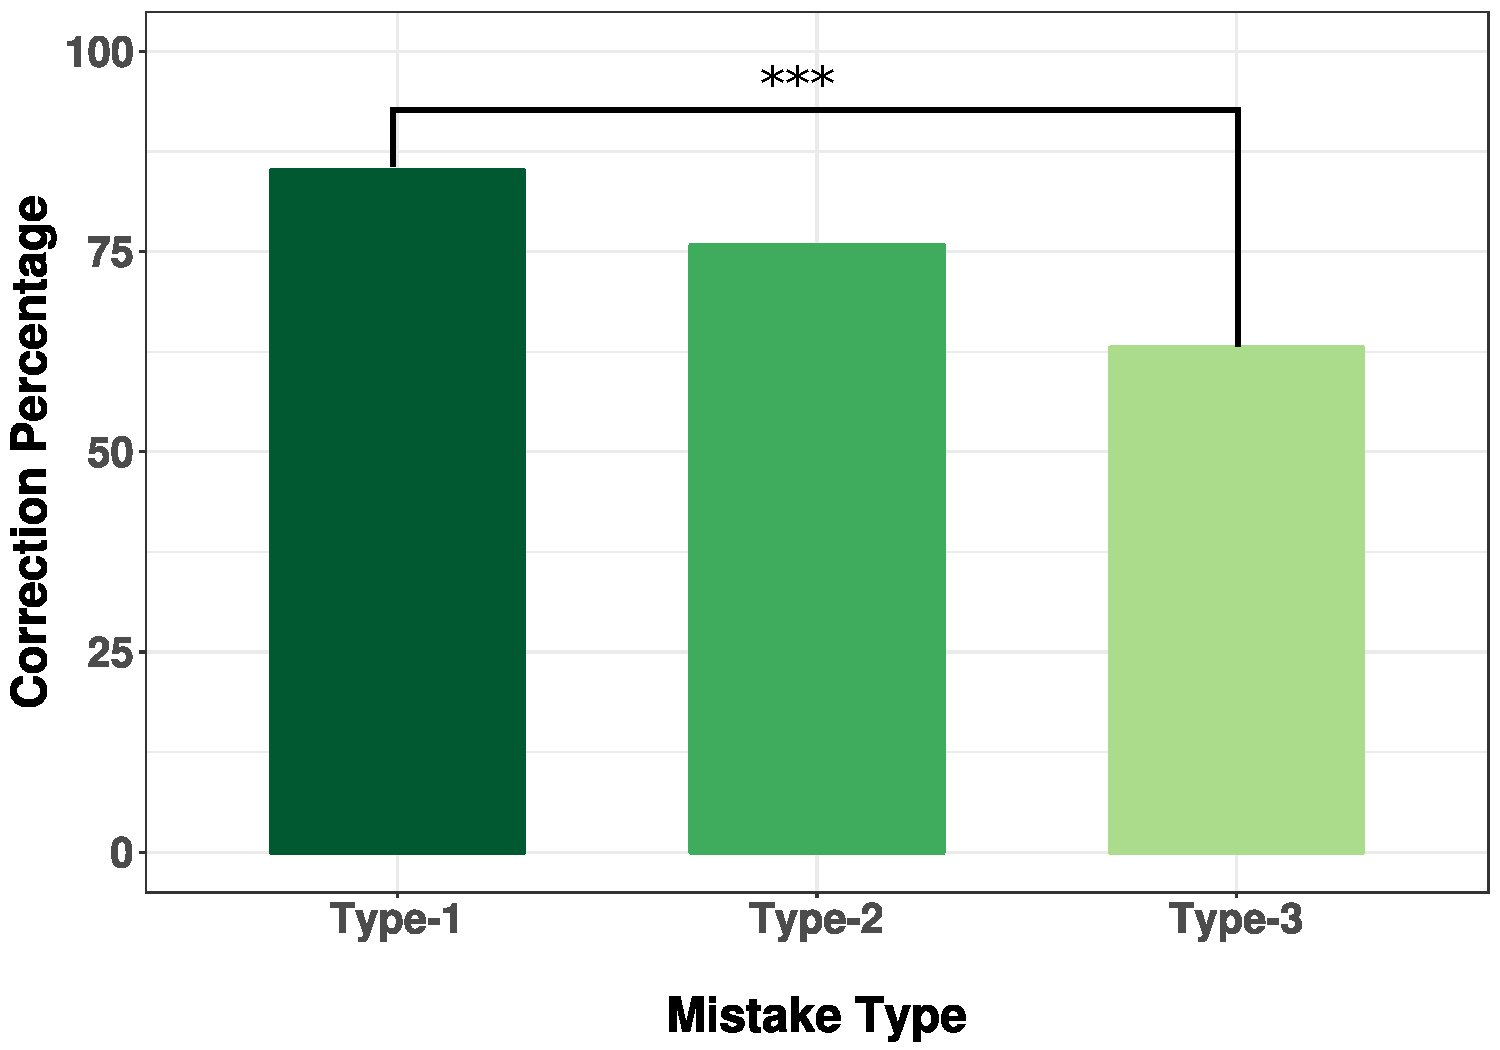
\includegraphics[width=1\linewidth]{figures/cVt.pdf}
  \caption{Validation check for the types of mistake. $***p<0.001$.}
  \label{fig:MistakeCor}
\end{figure}



\section{Results}

On the first day of study, 22 children participated in the experiment.
However, on the second day, 2 children from the Low-level group and 2 children from the High-level group were absent.
Furthermore, 2 children from the 18 participants who repeated the experiment were removed due to loss of data logs.
The final results are obtained from 16 participants.
Considering the within-subject design of the experiment, we checked if there was any effect between the first and second day of the experiment.
The analyses shows no significant difference between days $(\chi^2 = 0.5537, df = 1, p-value = 0.4568)$.

\subsection{H1: Effect of Pointing on Correction}
Figure \ref{fig:Pointing} shows the correction percentage according to the pointing conditions.
Pearson's Chi-squared test with Yates' continuity correction is used to evaluate the difference between the two conditions.
This test shows no significant difference between pointing and not pointing conditions $(\chi^2 = 0.68952, df = 1, p-value = 0.4063)$.
Considering that our main hypothesis is to show that pointing improves children's performance in reading and recognizing the mistakes, no significant difference is observed, hence our first hypothesis is rejected. 

\begin{figure}[t]
  \centering
  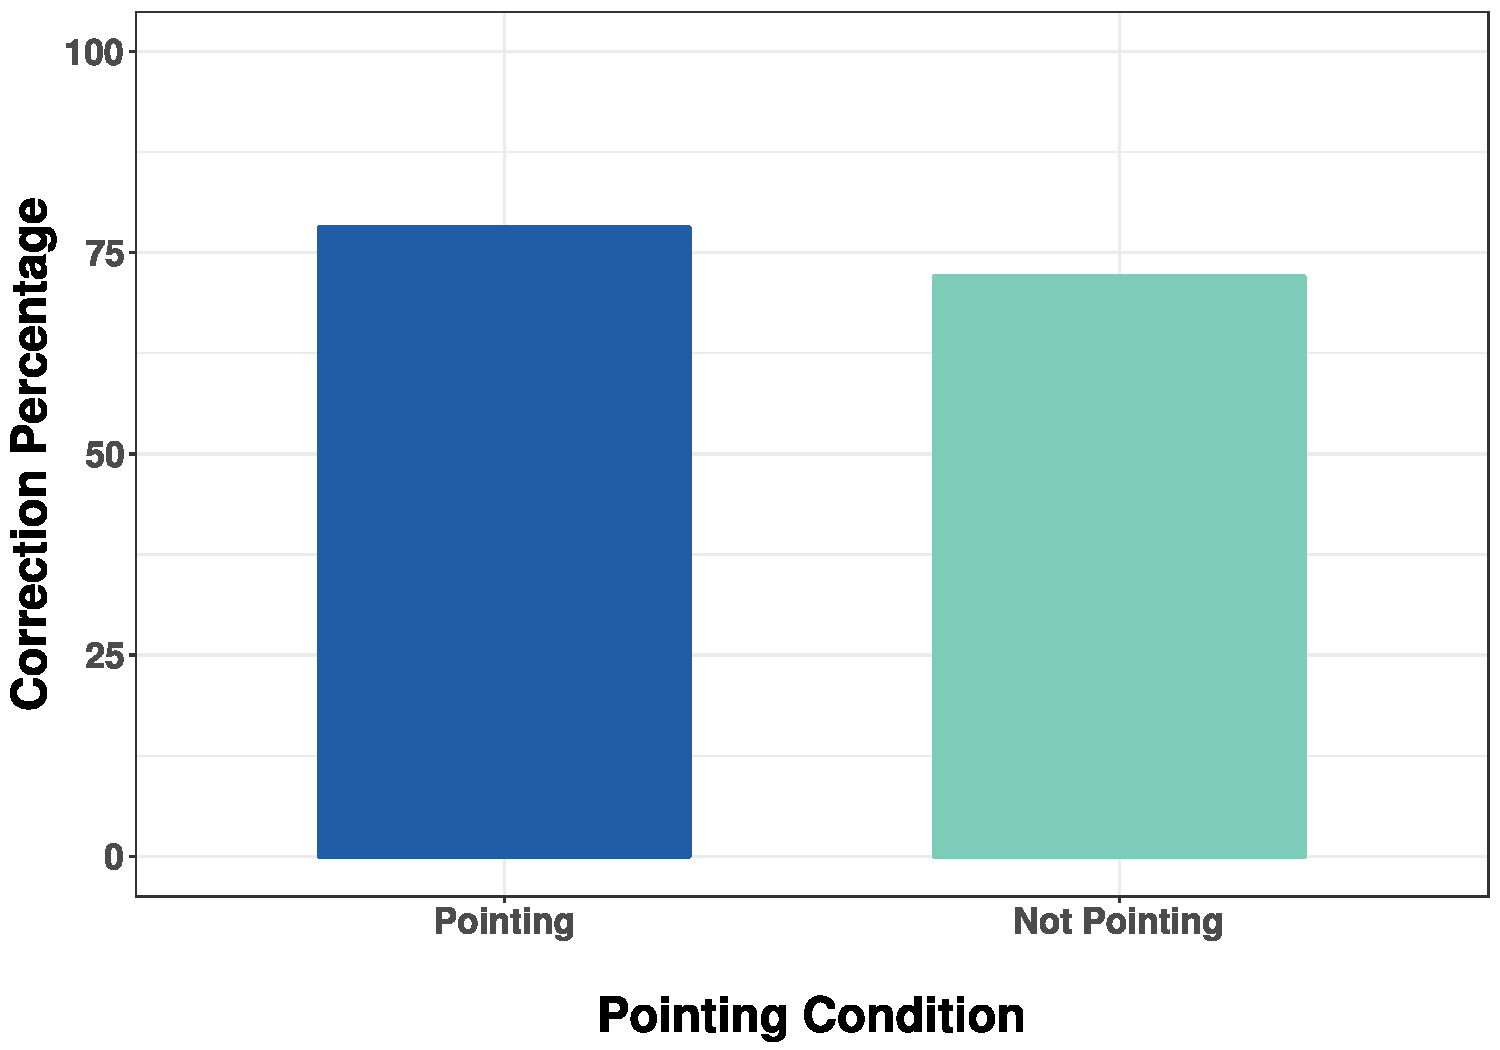
\includegraphics[width=1\linewidth]{figures/cVp.pdf}
  \caption{Performance according to correction percentage measure divided based on pointing conditions.}
  \label{fig:Pointing}
\end{figure}

\subsection{H2: Interaction Between Pointing and Mistake Type}
Figure \ref{fig:PointingVsType} demonstrates the correction percentage for each type of mistake for both pointing conditions. 
In particular, the interaction between mistake types and pointing conditions is presented here. 
We can observe that children in the pointing condition show much higher performances in correcting Type-1 mistakes.
This difference in performances for Type-1 mistakes is significant based on Pearson's Chi-squared test $(\chi^2 = 11.389, df = 1, p-value = 0.0007388)$.
This result proves our second hypothesis that pointing gesture is most effective on the mistakes recognizable through illustrations.
The differences for Type-2 and Type-3 mistakes between two pointing conditions are not significant with following test results $(\chi^2 = 0.19996, df = 1, p-value = 0.6548)$ and $(\chi^2 = 0.53361, df = 1, p-value = 0.4651)$ respectively.
Nevertheless, we will still explore the interaction between pointing conditions and mistakes types in more detail in the next section when we also group the result based on the children's reading level.



\begin{figure}[t]
  \centering
  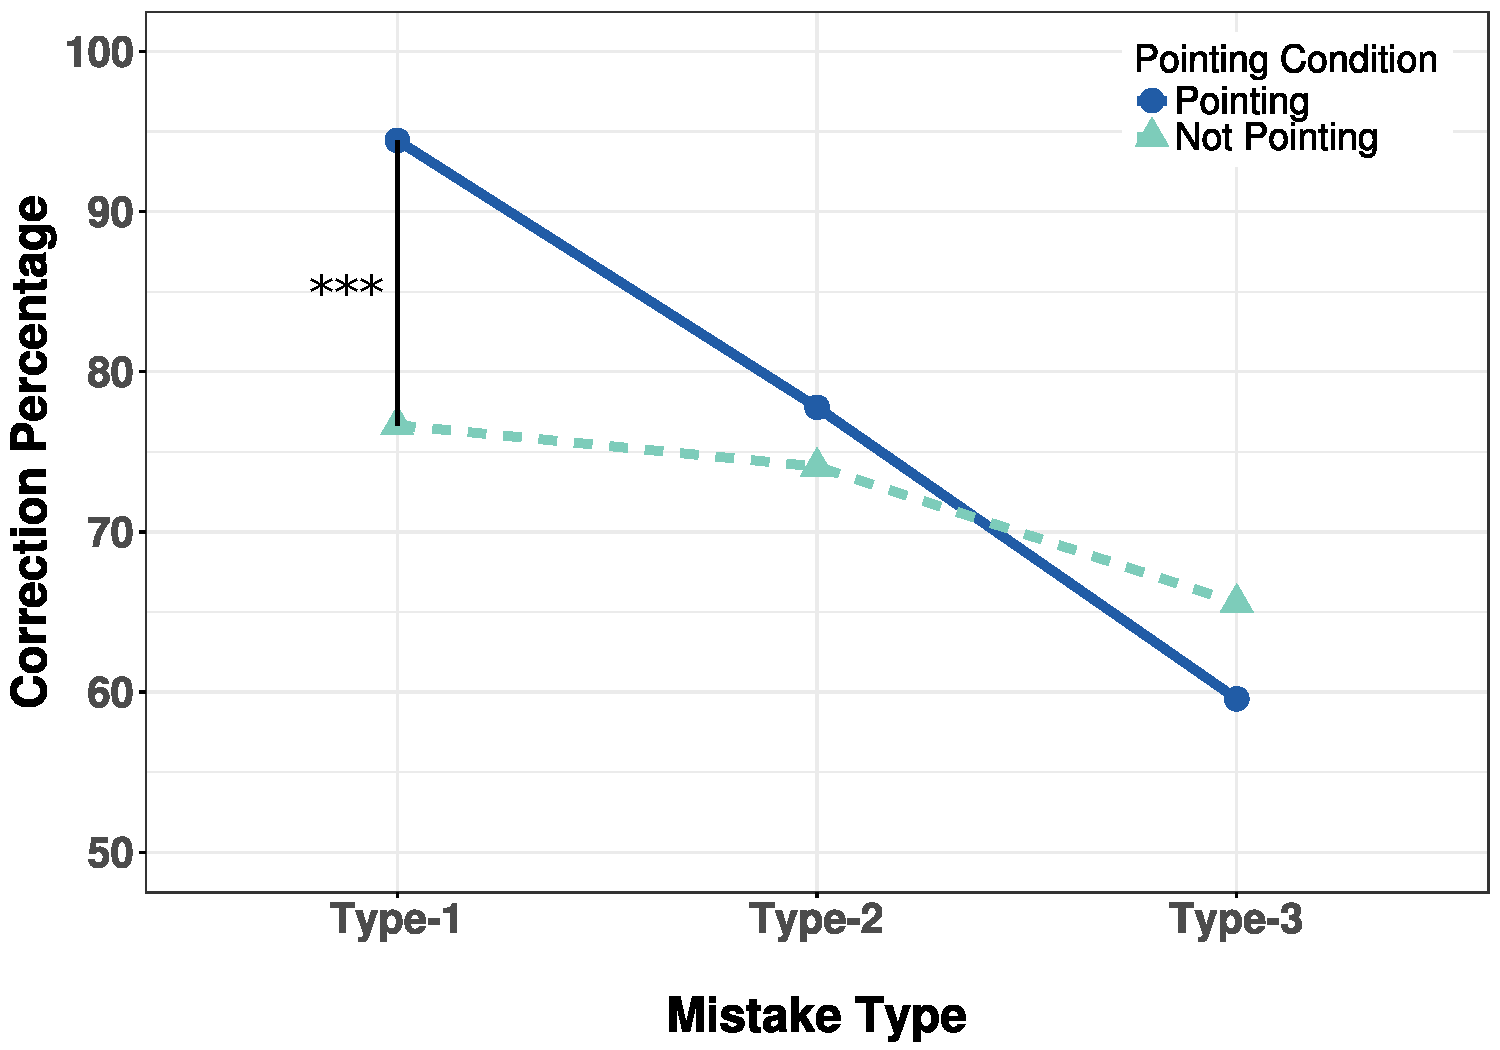
\includegraphics[width=1\linewidth]{figures/cVmVp2.pdf}
  \caption{Interaction Between pointing conditions and mistake types. $***p<0.001$.}
  \label{fig:PointingVsType}
\end{figure}   

\subsection{H3: Interaction Between Pointing and Reading Level}
In this section, we divide the results based on the children's reading level.
We have already discussed the interaction between pointing conditions and mistake types for all of the children in Figure \ref{fig:PointingVsType}.
In Figure \ref{fig:PointingVsTypeVsLevel}, we present the interaction between the pointing conditions and mistake types separated according to High and Low-levels. 


Figure \ref{fig:HighPointingVsTypeVsLevel}, for High-level group, shows that children in the pointing condition are more successful in correcting the robot when it makes Type-1 and Type-2 mistakes.
Pearson's Chi-squared test shows a significance of $*p<0.05$ for both Type-1 and Type-2 mistakes with $(\chi^2 = 4.2741, df = 1, p-value = 0.0387)$ and $(\chi^2 = 6.1791, df = 1, p-value = 0.01293)$ respectively.
The success in correcting the Type-1 mistakes corresponds to our second hypothesis.
And for Type-2 mistakes, we can say that pointing could have helped the High-level children to be more concentrated on the story and context. 
There is no significant difference in correcting Type-3 mistakes between the two pointing conditions $(\chi^2 = 0, df = 1, p-value = 1)$.
We can deduce that children who are proficient in reading benefit more from the pointing condition in correcting Type-1 and Type-2 mistakes. 



\begin{figure*}[t]
\centering
\begin{subfigure}{.48\textwidth}
  \centering
  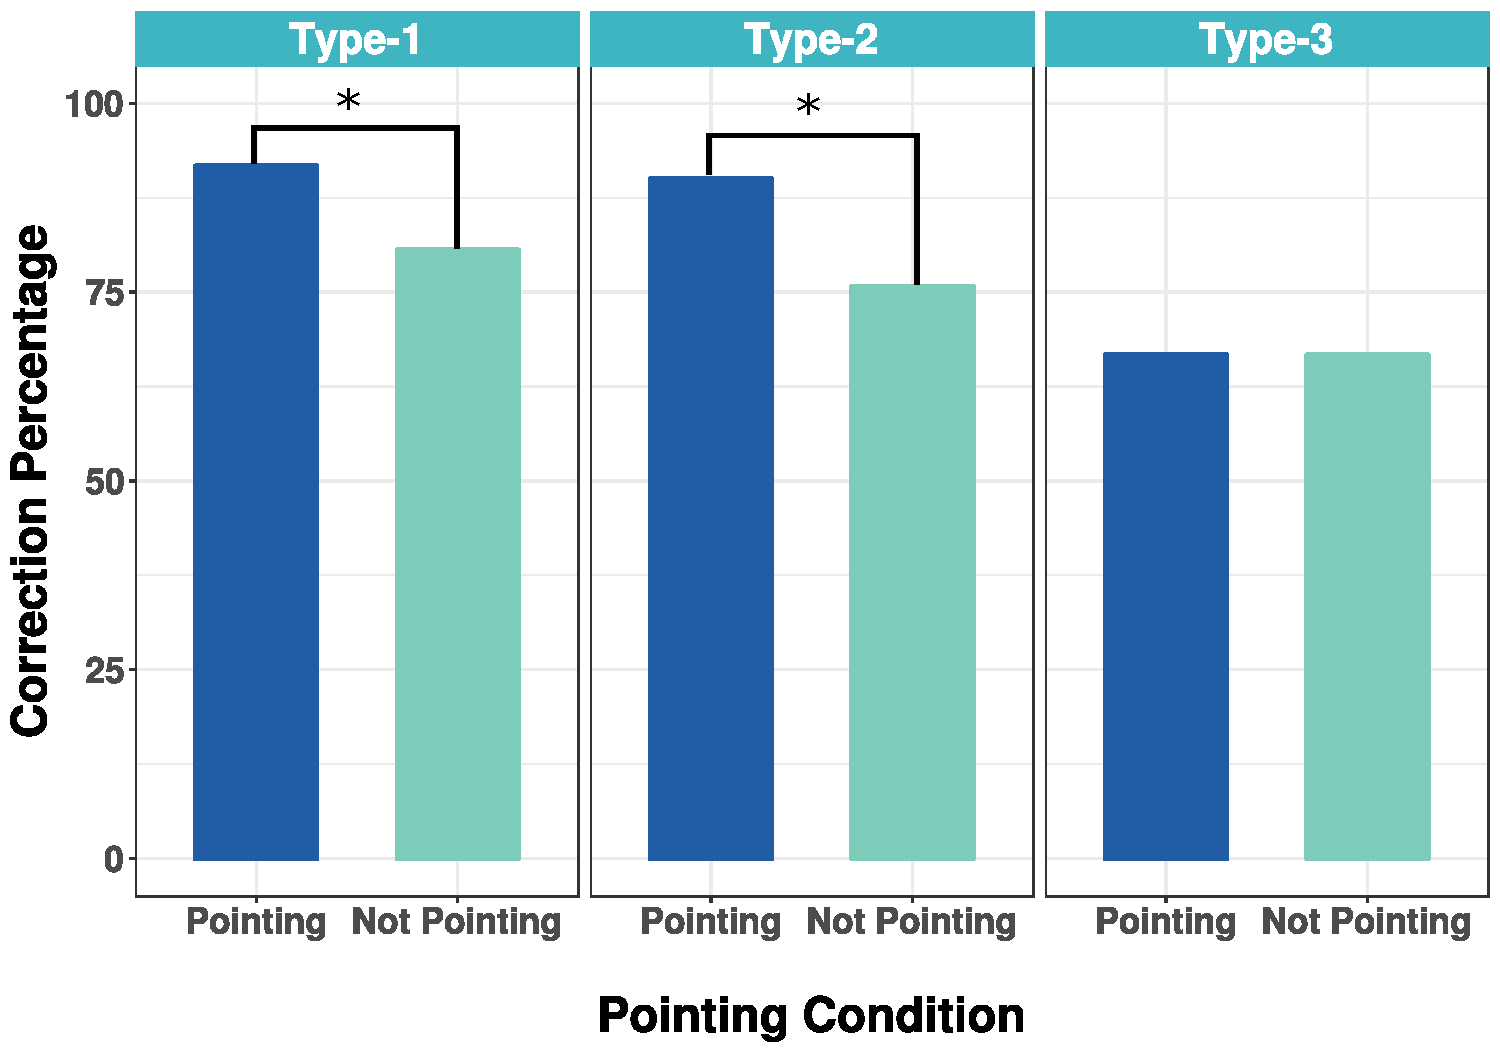
\includegraphics[width=0.95\linewidth]{figures/HcVpVt.pdf}
  \caption{High level group. $*p<0.05$}
  \label{fig:HighPointingVsTypeVsLevel}
\end{subfigure}%
\begin{subfigure}{.48\textwidth}
  \centering
  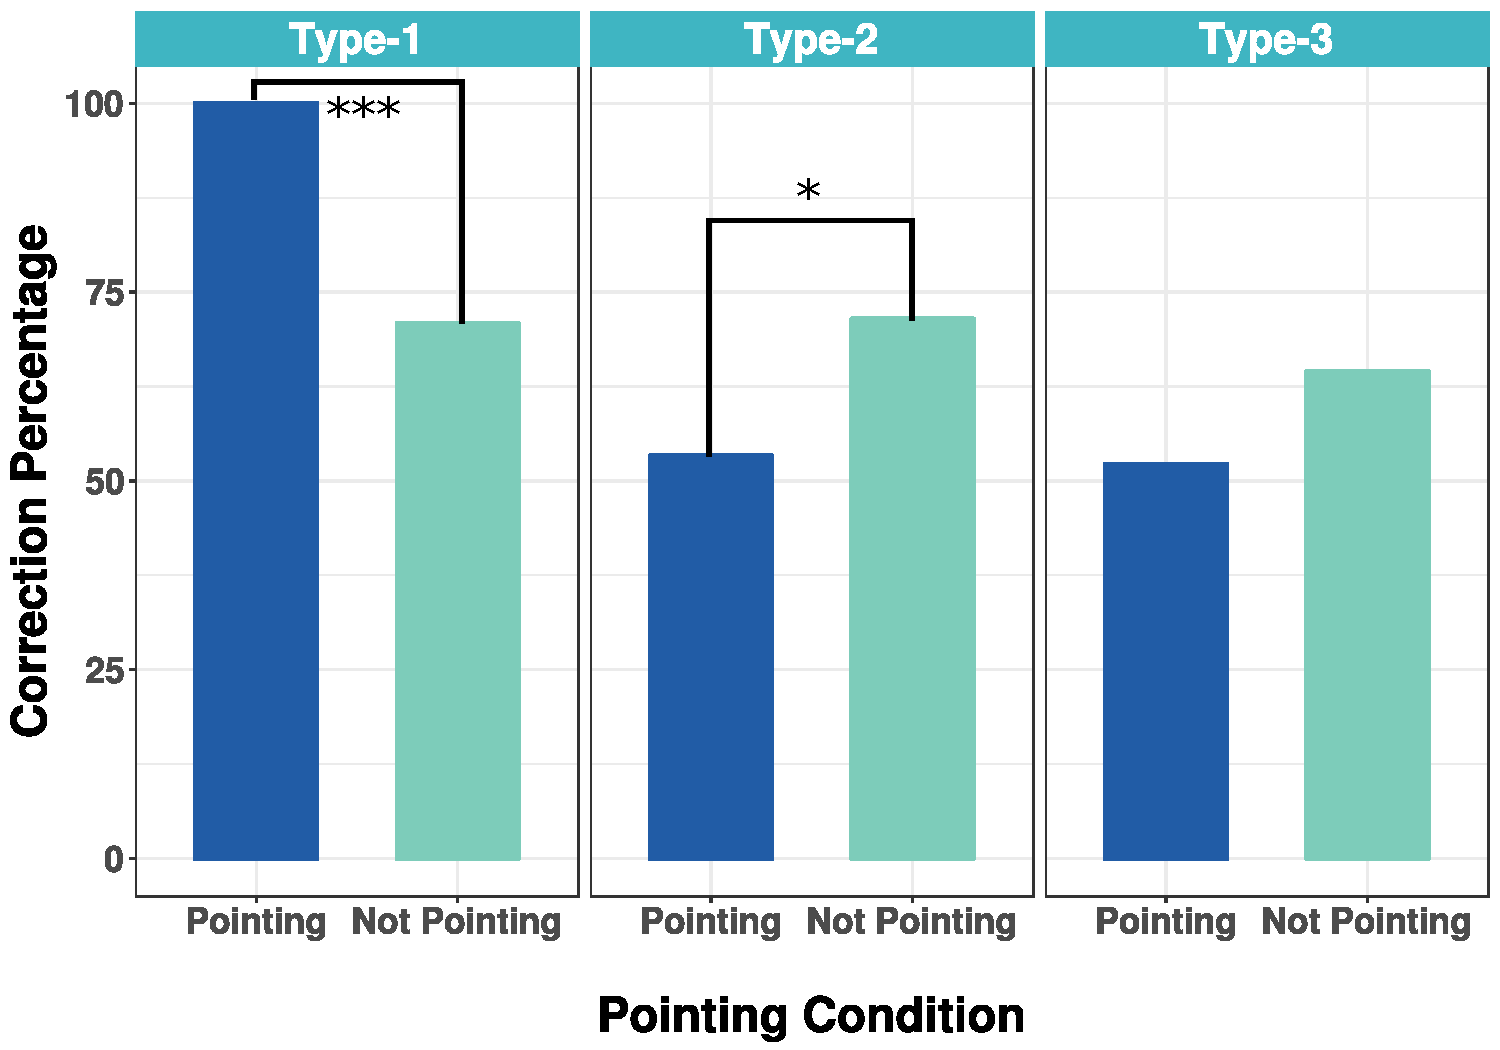
\includegraphics[width=0.95\linewidth]{figures/LcVpVt.pdf}
  \caption{Low level group. $*p<0.05$ and $***p<0.001$}
  \label{fig:LowPointingVsTypeVsLevel}
\end{subfigure}
\caption{Correction percentage for each type of mistake, arranged by pointing conditions; for High-level in the left figure and Low-level in the right figure.}
\label{fig:PointingVsTypeVsLevel}
\end{figure*}

Figure \ref{fig:LowPointingVsTypeVsLevel} shows the performance of the Low level group.
We observe that this group was differently affected by the pointing conditions. 
They showed a better performance for the Type-1 mistakes and lower performance for the Type-2 and Type-3 mistakes, in the pointing condition. 
In the pointing condition, children were significantly better in recognizing the Type-1 mistakes $(\chi-squared = 31.845, df = 1, p-value = 1.67e-08)$. 
This is aligned with the result of our second hypothesis.
However, surprisingly, pointing gestures had a negative effect on the recognition of Type-2 mistakes. 
The difference between the two conditions for Type-2 mistakes is significant with $*p<0.05$ using Chi-squared test $(\chi^2 = 6.2267, df = 1, p-value = 0.01258)$. As it will be discussed later, the justification can be that children in the Low-level group may have been distracted by the pointing gestures.
Moreover, similar to the previous results, pointing doesn't have a significant effect on children finding Type-3 mistakes $(\chi^2 = 2.6466, df = 1, p-value = 0.1038)$.

We can conclude that children at both levels can benefit from pointing gestures when having to recognize mistakes that are a mismatch with the image.
However, pointing seems to distract children in the Low-level group from comprehending the text.
And as a result, in the pointing condition, they achieved a lower performance in recognizing mistakes when there was a mismatch with the meaning of the text.





\section{Discussions}

\subsection{Pointing Gestures}
The main goal of this study is to evaluate the effect of pointing gesture by a robot in a reading activity with a child peer. 
The result from our user study shows that overall the pointing has some significant, yet diverse, effects on the children's reading, and particularly on their capability to detect and correct the robot's mistakes. 
Our findings are aligned with the results from Justice et al. \cite{justice2008influence}, that explicit referencing to the print such as pointing increases the children visual attention to the print.
However, we notice that the pointing affects mistake recognition differently based on the type of mistake and based on the children's proficiency in reading.
We observed that pointing has a significant effect in recognizing the mistakes that are a mismatch between text and images, for both reading levels. 
The effect on this type of mistakes is more significant for early readers compared to children who are more proficient in reading. 
On the other hand, for the mistakes that are a mismatch between text and meaning, pointing has a different effect on children in Low-level compared to High-level.
While pointing helps children with High-level proficiency to recognize the mistakes related to the meaning, it has a significantly negative effect on Low-level children.
Presumably, while the robot pointing gesture brings the child's attention to the images, it may also distract them from comprehending the context, thus leading to a negative result. 
This can also be confirmed from the observations made, that some children in the pointing condition were actually looking at the robot's hand and were curious about it, rather than following the story and its reading.
Subsequently, pointing does not have a significant overall positive effect on recognizing mistakes that are a mismatch with pronunciation or syntax.

\subsection{Teachers' Input}
One important aspect of this type of studies is the teachers' feedback. 
In general, the teachers were really cooperative and interested in the project. 
They were willing to let the experimenter attend the class to become more familiarized with the classroom and the methods they used.
When we explained about the general idea and the concept of the robot reading to the child, they were very positive and considered that challenging children with one level higher book was indeed a good idea.
Regarding the development and design of the mistakes, they provided us with relevant input about the common mistakes that children usually make during reading.
Their suggestions were incorporated into the design of the experiment.
There was also a suggestion about adding more modes of interaction between the child and the robot, and thus enrich the whole experience. 
The idea comes from the fact that when children have a problem reading a word, especially in the Low-level group, they start deciphering the word letter by letter and by sounding each letter.
Usually, when a child starts deciphering, they either recognize the word and read it successfully or they get help from the teacher to complete the word. 
Some new types of interaction that could help this process would be very useful. 
In fact, the proposed idea was to incorporate the deciphering mode into the robot and let the child be the one who would help the robot to read the word. 

\subsection{Children's Input}
Basing our study on the learning by teaching paradigm, we figured informing children of their role during the experiment is a fundamental component of this experiment. 
Children were aware that they would be helping and correcting the robot and they were pretty excited about the interaction, especially the idea of being a teacher for the robot.
Children were selected randomly from the class and had a one-to-one interaction with the robot. 
They were as excited about working with the robot in the second session as they were in the first one. 
After the end of the second session, nearly half of the students were asking about when there will be the next session. 
Some children were suggesting which book they want to read in the next session, with the statements such as
\textit{``Can we have another book, the other time? [experimenter: Yeah, sure what book do you like?] another adventure, I like adventures, about Gazelles, I love Gazelles, that's my favorite animal''}.
Or some children had a long interaction with the robot before they leave the room, about seeing it in the next session.
\textit{``Are you gonna have a third test? [Experimenter:not now] When will we have the third test, when everybody has the second test? [to the robot] See you in the third test''}.
Some of the interesting reactions from the children were about the robot's progress in reading and their concern that if the book was too hard for the robot.
Occasionally they were suggesting about how much the robot should practice reading by saying \textit{``He need to read easier books''} or \textit{``He get better if he reads 10 books [experimenter: In a day?] aaah... in a week''.}

Regarding the mistake types, children were sometimes amused by the Type-1 mistakes and for them, it was interesting that the robot makes such mistakes, yet they were very understanding about it.
In addition, while attending a reading session with the class, the experimenter had observed children with lower reading proficiency make similar types of mistakes.
As mentioned earlier, some mistakes were suggested by their teacher and inspired by the common mistakes that the children make during reading.
For these mistakes, some children were quick to figure out the association as they probably heard them before. 
For example, when the robot said \textit{saw} instead of \textit{was} there were cases who understood the robot is reading the word backward or mentioned some of their peers make similar mistakes.

\subsection{Limitations}
Our study has its own set of limitations, that should be considered in the interpretation of our findings. 
We explain these limitations here and how we try to overcome them, in our future development section.

\textbf{\textit{Limited number of participants:}}
We found the participants of this user study by first having pilots on the first and third graders, in order to improve our design and find the right audience.
As a result, we targeted one classroom in the second grade, to have a homogeneous level of children, considering different classes have different learning structures and speeds, and we wanted to have a comparable group of students.
However, we are fully aware that a larger number of participants gives more validity to the results. 
Our main goal is to train and develop our platform for a broad audience and users.
As a result, we will try to gradually expand our set of participants in the future studies.

\textbf{\textit{Limited number of reading sessions:}}
One of the goals of our platform is to provide a sustainable interaction. 
It is important to increase the number of sessions to observe the children's behavior over the sessions.
We are aware that children's performances, in the first few sessions, can be affected by the novelty effect of using a robot.
Due to limitations imposed by other factors and school curriculum, we were only able to have two sessions per child in this user study.
However, we are trying to develop a more sustainable system for long-term interactions.
By upgrading the system, providing a more robust learning objectives, and integrating the inputs from previous studies, teachers, and children we can plan for long-term user studies.

\textbf{\textit{Limited modes of interaction:}}
In this user study, we only had one mode of interaction and one measure which was correcting the robot. 
We are planning to develop and integrate new modes of interaction in our future studies.
We have already tried using one mode of interaction that requires speech recognition in one of our pilot studies. 
Considering this mode requires more development and preparation, due to issues with speech recognition for children, we will try to work around it for our future developments.
Our suggestions and plans to increase the modes of interactions will be discussed in more detail in the future development section.

\textbf{\textit{Fixed mistakes:}}
In the current experiment, the mistakes were designed by the experimenter following our design guidelines.
The goal was to test our design structure for creating and implementing the mistakes into the system in order to evaluate and improve it for future.
We will make the design of the mistakes more automated in the future, and try to generate an algorithm that is adjustable to different factors such as difficulty and the child's level.


\textbf{\textit{Scripted interaction:}}
The current interaction was autonomous and scripted, which can work for a limited number of sessions.
But, by increasing the number of sessions, we need to make the robot's behavior more diverse and flexible.
The idea is to expand the range of the robot's behaviors in conjugation with the new modes of interaction.



\subsection{Future Developments}
This platform is designed with the idea of providing a reading companion for children. 
It is supposed to be complementary to their existing practices and accompanies them in early stages of learning, especially for children with reading difficulties.
Based on the user study and our goals, there are four main development points that we are willing to make.

\textbf{\textit{Developing Adaptive Pointing:}}
Our observations and results from the user study show that continuous pointing gesture has diverse effects on the children's attention to reading.
While it can be constructive in some aspects, it can also be distractive in some other aspects. 
As a result, we decided to design an adaptive pointing system based on the positive and negative effects of pointing.
According to our observations, sometimes children in not pointing group were getting lost not knowing which page the robot was reading.
As a result, they either asked the robot to repeat or considered it as a mistake.
For these reasons, we will keep the pointing as a more informative gesture from the robot to inform the child on the correct page, to bring the child's attention to reading when they are distracted, and to point at words that are harder to read.

\textbf{\textit{Increasing Modes of Interaction:}}
Considering that correcting the robot's mistake is just one mode of interaction, we have lots of possibilities to design other modes of interaction in this context. 
These new modes can be inspired by the children's reading habits, such as when they decipher the text to read a new word, or when they ask someone else to read a word for them. 
We have already designed the version when the robot sometimes asks the child to read a word, but we haven't included it in our current user-study due to issues with speech recognition for children.
However, we are planning to integrate this mode into our future interactions. 
Another mode of interaction would be when the robot starts deciphering the word and hesitates to read it, in order for the child to help the robot to pronounce the word correctly.
These new modes of interaction may need their own deictic gestures, which can be more informative and different from the continuous pointing gesture we tested in this study. 

\textbf{\textit{Adapting the Mistakes to the Child's Level:}}
One important aspect of this interaction is the children's perception of being the teacher. Therefore, when the child corrects the robot, it seems essential that the robot shows some improvements. 
In the current study, as a design feature, the robot doesn't make any mistake on the last page in each session, to give the impression of improvement to the child.
We would like to make two main improvements to the system directed to this aspect.
First, to adapt the mistakes types and difficulty to the child's level of reading. 
This can be achieved by analyzing the child's reading style using eye-tracking in an initial reading or by the type of mistakes he/she makes during reading.
Moreover, we can also customize the mistakes to the types that the child does or does not recognize.
Such adapting system can also help the robot to switch between different modes based on the child's strengths and weaknesses, to challenge them more.
Second, to adjust the number of mistakes based on the child's performance in real-time. 
Especially to decrease the number of mistakes or certain types of them when the child has a good performance to give an illusion of improvement in the robot.

\textbf{\textit{Integrating Eye-Trackers:}}
Having adaptive pointing gestures call for providing more information to the robot regarding the child's real-time attentional state.
Robot's knowledge of the child's attentional state can help it in achieving joint attention. 
There have been numerous studies on joint attention between human and a robot.
A robot with such a knowledge is able to initiate joint attention (IJA) with the child, respond to joint attention (RJA) cues from the child, and ensure it (EJA) during the interaction.
As a result, the interaction becomes more robust and autonomous. 
For these reasons, we are interested in using eye-tracking glasses and integrating eye-tracking data into our robot. 
Such implementation consequently benefits our previous remarks on the future development of our platform.



\section{Conclusions}
Our work builds upon a growing body of literature on robotics in education, in more detail as a learning companion and particularly reading activities. 
We tried to understand the building blocks of reading as a fundamental skill and suggest an interaction model inspired by miscue analyses in reading. 
Furthermore, we tried to channel the learning by teaching paradigm as a way to keep children motivated to engage in the reading activity and to become more responsible for the robot. 
The main contribution of our study is to provide an understanding of the effect of pointing on reading in similar scenarios.
In order to help children in early stages of reading or with difficulties, it is essential to provide certain type of assistance only after careful examination regarding its effects.
We have observed, deictic gestures such as pointing affect children differently based on their reading proficiency. 
Pointing gestures can be beneficial for children in directing their attention to illustrations and helping them correcting mistakes associated with that.
However, we can conclude that pointing gestures might be distracting for children with low reading proficiency, preventing them from comprehending the text and recognizing mistakes related to that.

\section{Selection and Participation of Children}
22  children,  aged  6  to  7,  participated  in  the  study  reported in  this  paper.  All  of  them  were  from  the same school and 
were  recruited  from teachers who showed interest in project. 
All  students  provided  verbal  assent  to  participate when  the  Co-Reader  activities  were  initially  described  by their teachers,  and  parents  signed  consent  forms  prior  to video  and  audio  data  collection. 
Institutional recommendations were followed to insure data anonymization of all logged data.


\section{Acknowledgments}
This work was supported by national funds through Fundação para a Ciência e a Tecnologia (FCT) with reference UID/CEC/50021/2013. 
We would like to thank the Swiss National Science Foundation for supporting this project through the National Center of Competence in Research Robotics. 
Most importantly, We would like to show our gratitude toward Patrick Jefford, Justine Fisher, Nathan John Hobson and staff of primary section of International School of Geneva for their participation, support, and understanding through these experiments. With special thanks to all the children who participated in our experiment being so enthusiastic and caring to help our robot.   

% Balancing columns in a ref list is a bit of a pain because you
% either use a hack like flushend or balance, or manually insert
% a column break.  http://www.tex.ac.uk/cgi-bin/texfaq2html?label=balance
% multicols doesn't work because we're already in two-column mode,
% and flushend isn't awesome, so I choose balance.  See this
% for more info: http://cs.brown.edu/system/software/latex/doc/balance.pdf
%
% Note that in a perfect world balance wants to be in the first
% column of the last page.
%
% If balance doesn't work for you, you can remove that and
% hard-code a column break into the bbl file right before you
% submit:
%
% http://stackoverflow.com/questions/2149854/how-to-manually-equalize-columns-
% in-an-ieee-paper-if-using-bibtex
%
% Or, just remove \balance and give up on balancing the last page.
%
\balance{}

% BALANCE COLUMNS
\balance{}

% REFERENCES FORMAT
% References must be the same font size as other body text.
\bibliographystyle{unsrt}
\bibliography{reference.bib}
    
\end{document}

%%% Local Variables:
%%% mode: latex
%%% TeX-master: t
%%% End:
